\chapter*{Glosario}
\addcontentsline{toc}{chapter}{Glosario}

\begin{enumerate}
\item [Grafo] Un grafo, G, es un par ordenado de V y A, donde V es el conjunto de vértices o nodos del grafo y A es un conjunto de pares de vértices, a estos también se les llama arcos o ejes del grafo. Un vértice puede tener 0 o más aristas, pero toda arista debe unir exactamente a dos vértices.

Los grafos representan conjuntos de objetos que no tienen restricción de relación entre ellos. Un grafo puede representar varias cosas de la realidad cotidiana, tales como mapas de carreteras, vías férreas, circuitos eléctricos, etc.

La notación G = A (V, A) se utiliza comúnmente para identificar un grafo.

Los grafos se constituyen principalmente de dos partes: las aristas, vértices y los caminos que pueda contener el mismo grafo.

\begin{figure}[hbtp]
   \centering
    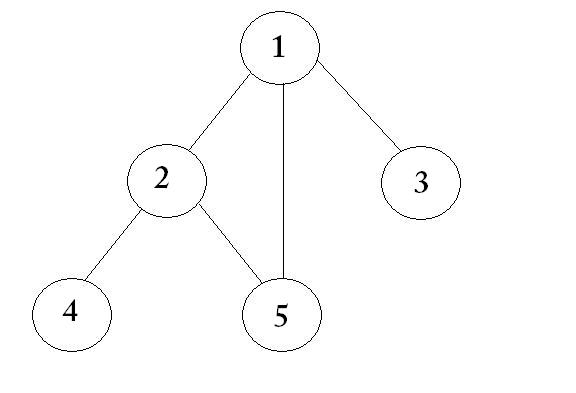
\includegraphics[scale=0.8]{images/grafo.png}
   \caption{Ejemplo de un grafo G, donde las Vértices(Nodos) son los círculos enumerados y los Arcos son las líneas que los unen }
    \end{figure}
\end{enumerate}
